%%% title presen240605
\documentclass[landscape,10pt]{jarticle}
\usepackage{pict2e}
\usepackage{ketpic2e,ketlayer2e}
\special{papersize=\the\paperwidth,\the\paperheight}
\usepackage{ketslide}
\usepackage{amsmath,amssymb}
\usepackage{bm,enumerate}
\usepackage[dvipdfmx]{graphicx}
\usepackage{color}
\usepackage[dvipdfmx,colorlinks=true,linkcolor=blue,filecolor=blue]{hyperref}
\usepackage{emath,emathE,emathMw}

\newcommand{\monthday}{0605}

\definecolor{slidecolora}{cmyk}{0.98,0.13,0,0.43}
\definecolor{slidecolorb}{cmyk}{0.2,0,0,0}
\definecolor{slidecolorc}{cmyk}{0.2,0,0,0}
\definecolor{slidecolord}{cmyk}{0.2,0,0,0}
\definecolor{slidecolore}{cmyk}{0,0,0,0.5}
\definecolor{slidecolorf}{cmyk}{0,0,0,0.5}
\definecolor{slidecolori}{cmyk}{0.98,0.13,0,0.43}
\def\setthin#1{\def\thin{#1}}
\setthin{0}
\newcounter{pagectr}
\setcounter{pagectr}{1}
\newcommand{\slidepage}[1][\monthday-]{%
\setcounter{ketpicctra}{18}%

\begin{layer}{118}{0}
\putnotew{130}{-\theketpicctra.05}{\small#1\thepage/\pageref{pageend}}
\end{layer}

}

\setmargin{25}{145}{15}{100}

\ketslideinit

\pagestyle{empty}

\begin{document}

\begin{layer}{120}{0}
\putnotese{0}{0}{{\Large\bf
\color[cmyk]{1,1,0,0}

\begin{layer}{120}{0}
{\Huge \putnotes{60}{20}{インストール状況}}
\putnotes{60}{50}{高遠節夫}
\end{layer}

}
}
\end{layer}

\def\mainslidetitley{22}
\def\ketcletter{slidecolora}
\def\ketcbox{slidecolorb}
\def\ketdbox{slidecolorc}
\def\ketcframe{slidecolord}
\def\ketcshadow{slidecolore}
\def\ketdshadow{slidecolorf}
\def\slidetitlex{6}
\def\slidetitlesize{1.3}
\def\mketcletter{slidecolori}
\def\mketcbox{yellow}
\def\mketdbox{yellow}
\def\mketcframe{yellow}
\def\mslidetitlex{62}
\def\mslidetitlesize{2}

\color{black}
\Large\bf\boldmath
\addtocounter{page}{-1}

\renewcommand{\slidepage}[1][s]{%
\setcounter{ketpicctra}{18}%
\if#1m \setcounter{ketpicctra}{1}\fi
\hypersetup{linkcolor=black}%
\begin{layer}{118}{0}
\putnotee{115}{-\theketpicctra.05}{\small\monthday-\thepage/\pageref{pageend}}
\end{layer}\hypersetup{linkcolor=blue}
}
%%%%%%%%%%%%

%%%%%%%%%%%%%%%%%%%%

\mainslide{インストール}


%%%%%%%%%%%%

%%%%%%%%%%%%%%%%%%%%

\newslide{前回の正弦曲線の結果}

\vspace*{18mm}

\slidepage
\textinit

\begin{layer}{120}{0}
\addtext{8}{\ten}{誤差の程度1.08-628.67}
\addtext{8}{\ten}{結果を見てみよう}
\end{layer}

%%%%%%%%%%%%

%%%%%%%%%%%%%%%%%%%%


\newslide{動作確認の状況}

\vspace*{18mm}

\slidepage
\textinit

\begin{layer}{120}{0}
\addtext{8}{\ten}{ketcindy(+日付)/template/01figure.cdy}
\putnotes{65}{20}{\scalebox{0.5}{%%% /Users/takatoosetsuo/specialclass.git/shibaura23/0621/fig/01figure.tex 
%%% Generator=01figure.cdy 
{\unitlength=1cm%
\begin{picture}%
(10.99,7.42)(-5,-4)%
\linethickness{0.008in}%%
\polyline(-5,0.132)(-4.963,0.311)(-4.927,0.479)(-4.89,0.631)(-4.853,0.761)(-4.817,0.867)%
(-4.78,0.943)(-4.744,0.988)(-4.707,1)(-4.67,0.978)(-4.634,0.924)(-4.597,0.838)(-4.56,0.725)%
(-4.524,0.587)(-4.487,0.43)(-4.45,0.258)(-4.414,0.078)(-4.377,-0.105)(-4.341,-0.284)%
(-4.304,-0.454)(-4.267,-0.609)(-4.231,-0.743)(-4.194,-0.853)(-4.157,-0.933)(-4.121,-0.983)%
(-4.084,-1)(-4.048,-0.983)(-4.011,-0.934)(-3.974,-0.853)(-3.938,-0.744)(-3.901,-0.61)%
(-3.864,-0.455)(-3.828,-0.285)(-3.791,-0.106)(-3.754,0.077)(-3.718,0.257)(-3.681,0.429)%
(-3.645,0.586)(-3.608,0.724)(-3.571,0.838)(-3.535,0.923)(-3.498,0.978)(-3.461,1)(-3.425,0.988)%
(-3.388,0.943)(-3.351,0.867)(-3.315,0.762)(-3.278,0.631)(-3.242,0.479)(-3.205,0.312)%
(-3.168,0.133)(-3.132,-0.049)(-3.095,-0.231)(-3.058,-0.404)(-3.022,-0.564)(-2.985,-0.705)%
(-2.949,-0.822)(-2.912,-0.912)(-2.875,-0.972)(-2.839,-0.998)(-2.802,-0.992)(-2.765,-0.952)%
(-2.729,-0.881)(-2.692,-0.78)(-2.655,-0.653)(-2.619,-0.504)(-2.582,-0.338)(-2.546,-0.161)%
(-2.509,0.022)(-2.472,0.203)(-2.436,0.378)(-2.399,0.541)(-2.362,0.685)(-2.326,0.806)%
(-2.289,0.9)(-2.252,0.965)(-2.216,0.996)(-2.179,0.995)(-2.143,0.96)(-2.106,0.893)%
(-2.069,0.797)(-2.033,0.673)(-1.996,0.527)(-1.959,0.364)(-1.923,0.188)(-1.886,0.006)%
(-1.85,-0.176)(-1.813,-0.353)(-1.776,-0.517)(-1.74,-0.664)(-1.703,-0.789)(-1.666,-0.888)%
(-1.63,-0.957)(-1.593,-0.994)(-1.556,-0.997)(-1.52,-0.968)(-1.483,-0.906)(-1.447,-0.813)%
(-1.41,-0.694)(-1.373,-0.551)(-1.337,-0.39)(-1.3,-0.215)(-1.263,-0.034)(-1.227,0.149)%
(-1.19,0.326)(-1.153,0.493)(-1.117,0.643)(-1.08,0.772)(-1.044,0.875)(-1.007,0.948)%
(-0.97,0.99)(-0.934,0.999)(-0.897,0.974)(-0.86,0.917)(-0.824,0.829)(-0.787,0.713)%
(-0.751,0.574)(-0.714,0.415)(-0.677,0.242)(-0.641,0.062)(-0.604,-0.121)(-0.567,-0.3)%
(-0.531,-0.469)(-0.494,-0.622)(-0.457,-0.754)(-0.421,-0.861)(-0.384,-0.939)(-0.348,-0.986)%
(-0.311,-1)(-0.274,-0.98)(-0.238,-0.928)(-0.201,-0.844)(-0.164,-0.733)(-0.128,-0.596)%
(-0.091,-0.44)(-0.054,-0.269)(-0.018,-0.089)(0.019,0.094)(0.055,0.273)(0.092,0.444)%
(0.129,0.6)(0.165,0.736)(0.202,0.847)(0.239,0.929)(0.275,0.981)(0.312,1)(0.348,0.985)%
(0.385,0.938)(0.422,0.859)(0.458,0.751)(0.495,0.618)(0.532,0.465)(0.568,0.296)(0.605,0.117)%
(0.642,-0.066)(0.678,-0.247)(0.715,-0.419)(0.751,-0.577)(0.788,-0.716)(0.825,-0.832)%
(0.861,-0.919)(0.898,-0.975)(0.935,-0.999)(0.971,-0.99)(1.008,-0.947)(1.045,-0.873)%
(1.081,-0.769)(1.118,-0.64)(1.154,-0.489)(1.191,-0.322)(1.228,-0.144)(1.264,0.038)%
(1.301,0.22)(1.338,0.394)(1.374,0.555)(1.411,0.697)(1.447,0.816)(1.484,0.908)(1.521,0.969)%
(1.557,0.998)(1.594,0.993)(1.631,0.956)(1.667,0.886)(1.704,0.787)(1.741,0.661)(1.777,0.513)%
(1.814,0.348)(1.85,0.172)(1.887,-0.011)(1.924,-0.193)(1.96,-0.368)(1.997,-0.531)(2.034,-0.677)%
(2.07,-0.799)(2.107,-0.896)(2.144,-0.962)(2.18,-0.995)(2.217,-0.996)(2.253,-0.963)%
(2.29,-0.898)(2.327,-0.803)(2.363,-0.682)(2.4,-0.537)(2.437,-0.374)(2.473,-0.199)%
(2.51,-0.017)(2.546,0.165)(2.583,0.342)(2.62,0.508)(2.656,0.656)(2.693,0.782)(2.73,0.883)%
(2.766,0.954)(2.803,0.992)(2.84,0.998)(2.876,0.97)(2.913,0.91)(2.949,0.82)(2.986,0.702)%
(3.023,0.56)(3.059,0.4)(3.096,0.226)(3.133,0.045)(3.169,-0.138)(3.206,-0.316)(3.242,-0.483)%
(3.279,-0.635)(3.316,-0.765)(3.352,-0.869)(3.389,-0.945)(3.426,-0.989)(3.462,-0.999)%
(3.499,-0.977)(3.536,-0.921)(3.572,-0.835)(3.609,-0.721)(3.645,-0.583)(3.682,-0.425)%
(3.719,-0.253)(3.755,-0.073)(3.792,0.11)(3.829,0.289)(3.865,0.459)(3.902,0.613)(3.939,0.747)%
(3.975,0.855)(4.012,0.935)(4.048,0.984)(4.085,1)(4.122,0.982)(4.158,0.932)(4.195,0.85)%
(4.232,0.74)(4.268,0.605)(4.305,0.45)(4.342,0.28)(4.378,0.1)(4.415,-0.083)(4.451,-0.263)%
(4.488,-0.434)(4.525,-0.591)(4.561,-0.728)(4.598,-0.841)(4.635,-0.925)(4.671,-0.979)%
(4.708,-1)(4.744,-0.987)(4.781,-0.942)(4.818,-0.864)(4.854,-0.758)(4.891,-0.627)(4.928,-0.475)%
(4.964,-0.306)(5.001,-0.128)(5.038,0.055)(5.074,0.236)(5.111,0.409)(5.147,0.568)(5.184,0.709)%
(5.221,0.825)(5.257,0.914)(5.294,0.973)(5.331,0.999)(5.367,0.991)(5.404,0.951)(5.44,0.878)%
(5.477,0.776)(5.514,0.648)(5.55,0.499)(5.587,0.333)(5.624,0.155)(5.66,-0.027)(5.697,-0.209)%
(5.734,-0.383)(5.77,-0.545)(5.807,-0.689)(5.843,-0.809)(5.88,-0.903)(5.917,-0.966)%
(5.953,-0.997)(5.99,-0.995)%
%
\polyline(-5,0)(5.99,0)%
%
\polyline(0,-4)(0,3.417)%
%
\settowidth{\Width}{$x$}\setlength{\Width}{0\Width}%
\settoheight{\Height}{$x$}\settodepth{\Depth}{$x$}\setlength{\Height}{-0.5\Height}\setlength{\Depth}{0.5\Depth}\addtolength{\Height}{\Depth}%
\put(  6.040,  0.000){\hspace*{\Width}\raisebox{\Height}{$x$}}%
%
\settowidth{\Width}{$y$}\setlength{\Width}{-0.5\Width}%
\settoheight{\Height}{$y$}\settodepth{\Depth}{$y$}\setlength{\Height}{\Depth}%
\put(  0.000,  3.470){\hspace*{\Width}\raisebox{\Height}{$y$}}%
%
\settowidth{\Width}{O}\setlength{\Width}{-1\Width}%
\settoheight{\Height}{O}\settodepth{\Depth}{O}\setlength{\Height}{-\Height}%
\put( -0.050, -0.050){\hspace*{\Width}\raisebox{\Height}{O}}%
%
\end{picture}}%}}
\addtext[50]{6}{問\monbannoadd}{上の図のPDFができたか}
\end{layer}

\addban
%%%%%%%%%%%%

%%%%%%%%%%%%%%%%%%%%


\newslide{ダウンロード}

\vspace*{18mm}

\slidepage
\textinit

\begin{layer}{120}{0}
\putnotese{40}{20}{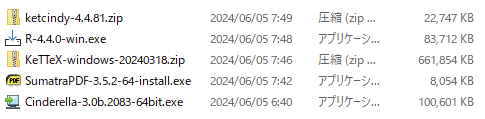
\includegraphics[bb=0 0 485 119,width=95mm]{fig/DLlist.png}}
\addtext{8}{\ten}{Sumatra(Windowsのみ)}
\addtext{8}{\ten}{R}
\addtext{8}{\ten}{Cinderella}
\addtext{8}{\ten}{KeTTeX}
\addtext{8}{\ten}{KeTCindy}
\addtext{6}{問\monbannoadd}{ダウンロードはすべて終わっているか}
\end{layer}

\addban
%%%%%%%%%%%%

%%%%%%%%%%%%%%%%%%%%


\newslide{インストール1}

\vspace*{18mm}

\slidepage
\textinit

\begin{layer}{120}{0}
\addtext{8}{\ten}{KeTCindyが動いていない時は再インストール}
\addtext{8}{\ten}{インストール済のファイルを削除しておく}
\addtext{8}{\ten}{Windows画面で説明}
\addtext{8}{\ten}{Sumatra}
\addtext{8}{\ten}{R}
\addtext{8}{\ten}{Cinderella}
\end{layer}

%%%%%%%%%%%%

%%%%%%%%%%%%%%%%%%%%


\newslide{KeTTeXのインストール}

\vspace*{18mm}

\slidepage
\textinit

\begin{layer}{120}{0}
\addtext{8}{\ten}{Windows画面で説明}
\end{layer}

%%%%%%%%%%%%

%%%%%%%%%%%%%%%%%%%%


\newslide{KeTCindyのインストール}

\vspace*{18mm}

\slidepage
\textinit

\begin{layer}{120}{0}
\addtext{8}{\ten}{Windows画面で説明}
\end{layer}

%%%%%%%%%%%%

%%%%%%%%%%%%%%%%%%%%


\newslide{動作確認}

\vspace*{18mm}

\slidepage
\textinit

\begin{layer}{120}{0}
\addtext{8}{\ten}{Windows画面で説明}
\end{layer}

\label{pageend}\mbox{}

\end{document}
